%%%%%%%%%%%%%%%%%%%%%%%%%%%%%%%%%%%%%%%%%
% Wenneker Assignment
% LaTeX Template
% Version 2.0 (12/1/2019)
%
% This template originates from:
% http://www.LaTeXTemplates.com
%
% Authors:
% Vel (vel@LaTeXTemplates.com)
% Frits Wenneker
%
% License:
% CC BY-NC-SA 3.0 (http://creativecommons.org/licenses/by-nc-sa/3.0/)
% 
%%%%%%%%%%%%%%%%%%%%%%%%%%%%%%%%%%%%%%%%%

%----------------------------------------------------------------------------------------
%	PACKAGES AND OTHER DOCUMENT CONFIGURATIONS
%----------------------------------------------------------------------------------------

\documentclass[11pt]{scrartcl} % Font size

%%%%%%%%%%%%%%%%%%%%%%%%%%%%%%%%%%%%%%%%%
% Wenneker Assignment
% Structure Specification File
% Version 2.0 (12/1/2019)
%
% This template originates from:
% http://www.LaTeXTemplates.com
%
% Authors:
% Vel (vel@LaTeXTemplates.com)
% Frits Wenneker
%
% License:
% CC BY-NC-SA 3.0 (http://creativecommons.org/licenses/by-nc-sa/3.0/)
% 
%%%%%%%%%%%%%%%%%%%%%%%%%%%%%%%%%%%%%%%%%

%----------------------------------------------------------------------------------------
%	PACKAGES AND OTHER DOCUMENT CONFIGURATIONS
%----------------------------------------------------------------------------------------

\usepackage{amsmath, amsfonts, amsthm} % Math packages

\usepackage{listings} % Code listings, with syntax highlighting

\usepackage[english]{babel} % English language hyphenation

\usepackage{graphicx} % Required for inserting images
\graphicspath{{Figures/}{./}} % Specifies where to look for included images (trailing slash required)

\usepackage{booktabs} % Required for better horizontal rules in tables

\numberwithin{equation}{section} % Number equations within sections (i.e. 1.1, 1.2, 2.1, 2.2 instead of 1, 2, 3, 4)
\numberwithin{figure}{section} % Number figures within sections (i.e. 1.1, 1.2, 2.1, 2.2 instead of 1, 2, 3, 4)
\numberwithin{table}{section} % Number tables within sections (i.e. 1.1, 1.2, 2.1, 2.2 instead of 1, 2, 3, 4)

\setlength\parindent{0pt} % Removes all indentation from paragraphs

\usepackage{enumitem} % Required for list customisation
\setlist{noitemsep} % No spacing between list items

%----------------------------------------------------------------------------------------
%	DOCUMENT MARGINS
%----------------------------------------------------------------------------------------

\usepackage{geometry} % Required for adjusting page dimensions and margins

\geometry{
	paper=a4paper, % Paper size, change to letterpaper for US letter size
	top=2.5cm, % Top margin
	bottom=3cm, % Bottom margin
	left=3cm, % Left margin
	right=3cm, % Right margin
	headheight=0.75cm, % Header height
	footskip=1.5cm, % Space from the bottom margin to the baseline of the footer
	headsep=0.75cm, % Space from the top margin to the baseline of the header
	%showframe, % Uncomment to show how the type block is set on the page
}

%----------------------------------------------------------------------------------------
%	FONTS
%----------------------------------------------------------------------------------------

\usepackage[utf8]{inputenc} % Required for inputting international characters
\usepackage[T1]{fontenc} % Use 8-bit encoding

\usepackage{fourier} % Use the Adobe Utopia font for the document

%----------------------------------------------------------------------------------------
%	SECTION TITLES
%----------------------------------------------------------------------------------------

\usepackage{sectsty} % Allows customising section commands

\sectionfont{\vspace{6pt}\centering\normalfont\scshape} % \section{} styling
\subsectionfont{\normalfont\bfseries} % \subsection{} styling
\subsubsectionfont{\normalfont\itshape} % \subsubsection{} styling
\paragraphfont{\normalfont\scshape} % \paragraph{} styling

%----------------------------------------------------------------------------------------
%	HEADERS AND FOOTERS
%----------------------------------------------------------------------------------------

\usepackage{scrlayer-scrpage} % Required for customising headers and footers

\ohead*{} % Right header
\ihead*{} % Left header
\chead*{} % Centre header

\ofoot*{} % Right footer
\ifoot*{} % Left footer
\cfoot*{\pagemark} % Centre footer
 % Include the file specifying the document structure and custom commands

%----------------------------------------------------------------------------------------
%	TITLE SECTION
%----------------------------------------------------------------------------------------
\title{	
	\normalfont\normalsize
	\textsc{Universidad Central del Ecuador}

	\textsc{Facultad de Ingeniería y Ciencias Aplicadas}

	\textsc{Carrera de Ingeniería Informática}
	\vspace{6pt} % Whitespace
	\rule{\linewidth}{0.5pt}\\ % Thin top horizontal rule
	\vspace{20pt} % Whitespace
	{\huge Informe de Servidor ETCD}\\ % The assignment title
	\vspace{12pt} % Whitespace
	\rule{\linewidth}{2pt}\\ % Thick bottom horizontal rule
	\vspace{12pt} % Whitespace
}

\author{\LARGE Nelson Ricardo Baquero} % Your name

\date{\normalsize\today} % Today's date (\today) or a custom date

\begin{document}

\maketitle % Print the title

\section{Servidor de Configuración ETCD}

\begin{figure}[h] % [h] forces the figure to be output where it is defined in the code (it suppresses floating)
	\centering
	
\includegraphics[width=0.5\columnwidth]{etcd-horizontal-color.png} % Example image
	\caption{Logo ETCD.}
\end{figure}

El etcd es un almacén de clave-valor open source, distribuido y uniforme que permite la configuración compartida, la detección de servicios y la coordinación del programador de clústeres o sistemas distribuidos de máquinas. Facilita la ejecución de actualizaciones automáticas de forma más segura, coordina el trabajo que se programa para los hosts e interviene en la configuración de las redes superpuestas para los contenedores.

%------------------------------------------------

\section{Instrucciones de instalación}

Las instrucciones de instalación son válidas para la mayoría de distribuciones de Linux.
Se utilizó \textbf{Fedora} en las capturas.

\subsection{Crear un script de instalación}

Crear un archivo llamado \emph{etcd-install.sh} con las siguientes instrucciones:

\begin{listing}[H]
	\inputminted[frame=lines,numbers=left]{bash}{etcd-install.sh}
	\caption{Contenido del archivo etcd-install.sh}
	\label{lst:install-script}
\end{listing}

Finalmente, otorgarle permiso de ejecución \mintinline{bash}{chmod +x etcd-install.sh}

\subsection{Ejecutar el script}

\begin{listing}[H]
	\begin{minted}[frame=lines]{bash}
$ ./etcd-install.sh
	\end{minted}
	\caption{Ejecución del script de instalación.}
	\label{lst:installation}
\end{listing}

Si la instalación resultó exitosa, ya es posible levantar el servidor.

\subsection{Desplegar el servidor ETCD}

Para desplegar el servidor, basta con ejecutar el binario (etcd):

\begin{listing}[H]
	\begin{minted}[frame=lines]{bash}
$ ETCD_BIN=/tmp/test-etcd
$ $ETCD_BIN/etcd
	\end{minted}
	\caption{Ejecución del binario.}
	\label{lst:execution}
\end{listing}

\subsection{Asignación de atributos clave/valor}

Finalmente, para agregar atributos clave/valor, se debe iniciar otra sesión de terminal y ejecutar el siguiente comando:

\begin{listing}[H]
	\begin{minted}[frame=lines]{bash}
$ $ETCD_BIN/etcdctl put [clave] [valor]
	\end{minted}
	\caption{Ingreso de un nuevo atributo.}
	\label{lst:input}
\end{listing}

Para obtener un valor a partir de su clave en la misma terminal, ejecutar el siguiente comando:

\begin{listing}[H]
	\begin{minted}[frame=lines]{bash}
$ $ETCD_BIN/etcdctl get [clave]
	\end{minted}
	\caption{Obtención de un atributo.}
	\label{lst:output}
\end{listing}

\section{Configuración en Java}

Utilizaremos un proyecto con Gradle como gestor de dependencias.

\subsection{Agregar las dependencias necesarias}

Se debe agregar las siguientes dependencias:

\begin{figure}[h] % [h] forces the figure to be output where it is defined in the code (it suppresses floating)
	\centering
	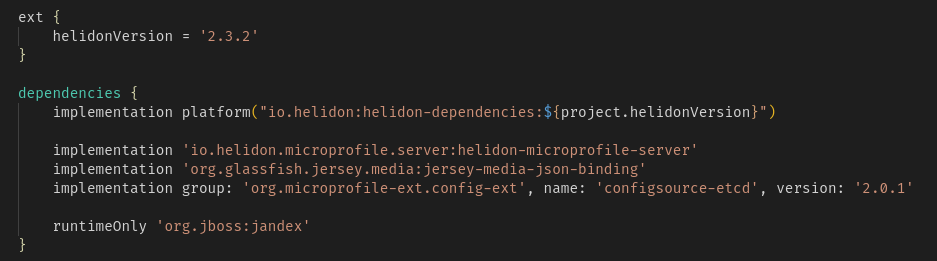
\includegraphics[width=1\columnwidth]{dependencies.png} % Example image
	\caption{Sección de dependencias en build.gradle}
\end{figure}

Además, debido a la antigüedad de una dependencia de la librería de configuración, se debe forzar a gradle a utilizar una versión anterior de la dependencia utilizando el siguiente código:

\begin{figure}[h] % [h] forces the figure to be output where it is defined in the code (it suppresses floating)
	\centering
	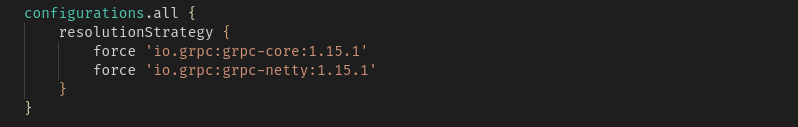
\includegraphics[width=1\columnwidth]{force.png} % Example image
	\caption{Sección de configuración en build.gradle}
\end{figure}

\subsection{Crear un archivo de configuración para ETCD}

El archivo debe tener como nombre \mintinline{bash}{microprofile-config.properties} y estar ubicado en el directorio \mintinline{bash}{META-INF} del proyecto.

Dentro del archivo se pueden colocar opciones de configuración como host, puerto, activar o desactivar, etre otras opciones.

\subsection{Utilizar los atributos de ETCD en el código}

Podemos utilizar CDI para inyectar los atributos. Por lo tanto necesitamos anotar la clase con un ámbito y anotar la propiedad que deseemos inyectar.

\begin{listing}[H]
	\begin{minted}[frame=lines,numbers=left]{java}
@ApplicationScoped // Anotación de ámbito
@Path("/")
public class HolaMundoRest {

  @Inject  // Anotación para inyectar una propiedad.
  @ConfigProperty(name = "app.mensaje2") // Anotación con la propiedad ETCD
  private String msg;

  @GET
  @Path("/hola")
  public String hola() {

    // Config providers
    ConfigProvider.getConfig().getConfigSources().forEach(s -> {
      System.out.printf("%3d: %s\n", s.getOrdinal(), s.getName());
    });

    return String.format("%s %s", msg, LocalDateTime.now());
  }
}
	\end{minted}
	\caption{Ejemplo de Hola Mundo utilizando configuración de ETCD.}
	\label{lst:java}
\end{listing}

\end{document}
